\documentclass[10.5pt]{report}
\usepackage[utf8]{inputenc}
\usepackage{nopageno}
\usepackage[top=2.5cm,bottom=2.5cm,left=2.5cm,right=2.5cm,bindingoffset=0.6cm]{geometry}

% Fuente Times New Roman
\usepackage{newtxtext,newtxmath}
% Tamaño de fuente específica
\usepackage{anyfontsize}
% Imágenes
\usepackage{graphicx}
% Justificar texto
\usepackage{ragged2e}
% Multiple columns
\usepackage{multicol,blindtext}
% Packages for tables
\usepackage{array}
\usepackage{longtable}
% Color for tables
\usepackage[table]{xcolor}
\usepackage{colortbl}

\begin{document}

\begin{center}
    \vspace*{1cm}
    
    {\fontsize{14}{16} \textbf{Prototipo embebido de la interpretación de patrones de movimiento en una mano para la reproducción de fonemas y palabras completas en el idioma Español de México}}
    
    \vspace{0.2cm}
    
    {\fontsize{12}{14} \textbf{\textit{Trabajo Terminal No. \_\_\_\_-\_\_\_}} }
    
    \vspace{0.1cm}
    
    \textit{Alumnos: *Valle Martínez Luis Eduardo}
    
    \vspace{0.1cm}
    
    \textit{Directores: Rodolfo Romero Herrera, Dr. Jesús Yaljá Montiél Pérez}
    
    \vspace{0.1cm}
    
    \textit{*e-mail: lvallem1400@alumno.ipn.mx}
    
\end{center}

\hfill\break
\justifying
\textbf{Resumen} - Las afectaciones del habla en adultos mayores suelen originarse después de una lesión o accidente comunmente con daño cerebral en el lóbulo izquierdo, limitando o completamente impidiendo la correcta comunicación verbal de las personas. Este proyecto propone un prototipo de \textit{wearable} y sistema embebido como herramienta de apoyo para pacientes con afectación del habla mediante la traducción de un código motriz con una mano a letras del alfabeto como texto y finalmente reproduciendo los fonemas de las palabras como discurso.

\hfill \break
\textbf{Palabras clave} - Afectaciones del habla, \textit{Machine Learning}, Sistemas Embebidos, \textit{Text-to-Speech}

\hfill \break
{\fontsize{12}{14}\textbf{1. Introducción}}
\hfill \break
\input{Secciones/Introducción}

\hfill \break
{\fontsize{12}{14}\textbf{2. Objetivo}}
\hfill \break
\justifying
\hfill\break 
Objetivo general: \hfill\break
Crear un sistema embebido como apoyo a la comunicación a personas con afecciones del habla conformado por un prototipo de \textit{wearable} sensor del movimiento en una mano, un modelo de \textit{Machine Learning} para la clasificación de los patrones y un servicio de \textit{Text-to-Speech} para la reproducción sonora de palabras y frases.

\hfill\break
Objetivos específicos:	
\begin{enumerate}

	\item \justifying Idear un conjunto de patrones de movimientos como código motriz que permita al usuario describir letras del alfabeto para la conformación de palabras y frases.
	
	\item \justifying Ensamblar el prototipo de guante \textit{wearable} sensor implementando el SoC micro:bit para el cambio de aceleraciones y un sensor de pulso para indicar el inicio y fin del muestreo de un movimiento.

	\item \justifying Identificar un modelo de \textit{Machine Learning} que en conjunto al algoritmo DTW clasifiquen eficientemente los patrones de movimiento a clases alfabéticas.
	
	\item \justifying Configurar el servicio local y en la nube de \textit{Text-to-Speech} para la reproducción sonora de las palabras y frases.
\end{enumerate}

\hfill \break
{\fontsize{12}{14}\textbf{3. Justificación}}
\hfill \break
\justifying
\hfill \break
\justifying
Las afectaciones en el habla en personas que han superado la etapa de niñez(adolescentes, adultos jóvenes, adultos y adultos mayores) suelen originarse principalmente por accidentes o lesiones que dañaron alguna zona de la masa encefálica, más comunmente afectando las funciones del lenguaje cuando se localiza en el hemisferio izquierdo del cerebro, ya sea por la falta de circulación del torrente sanguíneo, daño directo en las conexiones entre hemisferios, etc[7]. Se han estudiado para estas condiciones sus diferentes ramificaciones[7], mencionándose aquellas reconocidas como las que encontrarían mayor beneficio en el trabajo propuesto:
\begin{itemize}
	%
	%	Afasias
	%
	\item \textbf{Afasias}:
		\begin{itemize}
			\item \textbf{Afasia de Broca}[9,10]: El área de Broca es una región localizada en el lóbulo cerebral izquierdo y está relacionada con el uso del lenguaje. Específicamente la afasia en la que se sufre un daño en esta área, tienen dificultad para la expresión fluida, la pronunciación y modulación del tono de voz. La producción de los sonidos correctos y encontrar las palabras correctas suelen ser trabajos laboriosos, sin embargo la compresión del habla de otras personas es relativamente buena, por lo que entender textos o lenguaje oral en comparación con su capacidad de hablar y escribir se encuentra mejor conservada.
			\item \textbf{Afasia motora transcortical}[9]: Parecida a la afasia de Broca en la dificultad del paciente para la emisión de un lenguaje fluido y coherente conservando una relativa buena compresión de lenguaje, esta afectación difiere en el hecho de que los pacientes si son capaces de repetir lo que se les dice, mientras que aquellos que sufren de afasia de Broca son incapaces de repetir frases.
		\end{itemize}
	%
	%	Apraxia
	%
	\item \textbf{Apraxia:}
	\begin{itemize}
		\item \textbf{Apraxia bucofacial u orofacial}[11]: Incapacidad de realizar movimientos faciales a voluntad, como pasar la lengua por los labios, silbar, toser o guiñar el ojo.
		\item \textbf{Apraxia Verbal}[11]: Dificultad para coordinar los movimientos de la boca y del habla
	\end{itemize}
	%
	% 	Disartria
	%
	\item \textbf{Disartria}: Trastorno de la ejecución motora del habla, derivado de un problema neurológico debido a la presencia de un accidente cerebrovascular, traumas craneoencefálicos u otras lesiones cerebrales.[7] \\ Entre los síntomas se tienen el habla entrecortada jadeante, irregular, imprecisa o monótona, lenta, o rápida y "entre dientes", entonación anormal, cambios del timbre del voz, ronquera, babeo o escaces del control de la saliva y la movilidad limitada de la lengua, los labios y la mándibula.[13,14]
\end{itemize}

\hfill \break
\justifying
Buscando proporcionar una herramienta de apoyo para la comunicación a pacientes que han recientemente sufrido alguna accidente u lesión como las mencionadas anteriormente, no se enfoca el proyecto a un grupo de la sociedad con un amplio desarrollo del lenguaje de señas tal como suele ser común con las personas sordomudas. Esta propuesta consiste en un prototipo simplificado, apoyado en la idea de un sujetador de los dispositivos hardware con orificios para los dedos tipo \textit{wearable} y no un guante completo. De esta manera el componente principal de sensado, el SoC micro:bit, se encuentra en el dorso de la mano por lo que no interfiere de otra forma en la sensibilidad, o limitación motriz de los dedos. Todo esto hace al prototipo sencillo de usar, además de ser estético con la implementación de leds del SoC para indicar ciertas acciones, volviendolo también sencillo en la interacción.

\hfill \break
\justifying
Precisamente y debido a la sencillez del prototipo, se utiliza unicamente el sensor acelerómetro, descartando el agregado de otro tipo de sensores como los de flexión etc.

\hfill\break
\justifying
La creación del lenguaje codificado en un contexto de patrones de movimiento, le servirá al usuario para indicar el sonido que desea sea reproducido, y debido a que la forma más intuitiva para la mayor parte de la población(cerca del 95\% de la población que es alfabeta en México[15]) la asociación de la pronunciación de las letras en las palabras es natural mediante la relación en su representación escrita, se descarta un desglose directo en fonémas de las letras o palabras, siendo prácticamente desconocido un marco referencial como el Alfabeto Fonético Internacional y las asignaciones de los sonidos propios del español.

\hfill \break
{\fontsize{12}{14}\textbf{4. Productos o Resultados esperados}}
\hfill \break
\justifying
\begin{enumerate}
	\item Prototipo de \textit{wearable} tipo guante para la portabilidad del SoC micro:bit como elemento sensor y preprocesador de los patrones de movimiento, así como principal interfaz de interacción con el usuario
	
	\item Sistema embebido con comunicación entre el prototipo sensor y la tarjeta de sonido:
	\begin{itemize}
		\item Prototipo sensor \textit{wearable}
		\item Mini PC Raspberry Pi 4
		\item Tarjeta de Sonido WM8960 de Waveshare
	\end{itemize}
	
	\item Modelo basado en \textit{Machine Learning} para el procesamiento y clasificación de los patrones de movimiento a las respectivas clases textuales(letras, sílabas o plabras)
	
	\item Configuración de al menos 2 voces femeninas y 2 voces masculinas en diferentes rangos de tono de voz y edad
	
	\item Documento de publicación con el desarrollo de la solución propuesta
\end{enumerate}

\begin{figure}[!h]
	\centering
	\includegraphics[width=19cm]{Imagenes/Diagrama_Arquitectura.png}
	\caption{Diagrama de la arquitectura del sistema completo considerando al prototipo de sensado, el mini PC RaspberryPi 4 y la tarjeta de Audio.\\ La línea punteada inidica una comunicación \textit{wireless} tipo Bluetooth entre el micro:bit y la Raspberry Pi 4}
	\label{Arquitectura}
\end{figure}

\newpage
\hfill \break
{\fontsize{12}{14}\textbf{5. Metodología}}
\hfill \break
\justifying
\hfill \break
\justifying
Inicialmente fue considerada una Metodología de Prototipos, que cuenta con características similares a la metodología final escogida, difieriendo fundamentalmente en la filosofía de un desarrollo acelerado que pueda ofrecer una visión previa del producto, requiriendo una costante integración con el fin de realizar pruebas con los clientes e ir realizando las modificaciones o ajustes necesarios para cumplir con los requisitos dispuestos. Este enfoque aunque práctico, puede facilmente caer en el error de perder de vista los compromisos de calidad y mantenimiento que se acordaron con el cliente, esto debido a las continuas pruebas presentadas al cliente lo que hace que el desarrollo se riga a base de prueba y error.

\hfill \break
\justifying
Se ha decantado el desarrollo del proyecto por una Metodología basada en Componentes, por la naturaleza modular de la solución y los diferentes nodos y componentes que pueden irse mejorando independiente a la conformación completa del producto. Importante mencionar que el desarrollo independiente de cada componente requiere una definición correcta de los medios de conexión y protocolos de comunicación, facilitando y promoviendo una exitosa integración de todos los componentes.

\hfill \break
\justifying
Este paradigma considera un progreso de forma evolutiva implementando muchas bondades del modelo en espiral, siendo una de las herramientas más beneficiosas y también las más problemáticas si no se aplican de forma correcta, el análisis de riesgos. La eficiente predicción de riesgos requiere de experiencia y habilidad derivada del conocimiento profundo de la problemática y la solución por aplicarse, lo que requirirá asesoría con especialistas en las tecnologías que se utilizarán y permitiendo disminuír la incertidumbre de la detección errada de los riesgos.

\hfill \break
\justifying
Entre los beneficios de la implementación de esta metodología se encuentra la simplificación de pruebas, pues estas son ejecutadas para cada uno de los componenetes antes de ser ensamblados en el conjunto. A su vez esto simplifica el mantenimiento general del sistema, así como su escala y propicia la calidad del sistema completo mejorando continuamente los componentes de forma independiente.

\hfill \break
\justifying
Finalmente resaltar la ventaja que aporta su cualidad incremental respecto a la búsqueda del modelo de aprendizaje automático, asegurando aquel con la mejor precisión de predicción y eficiencia en el desempeño durante su entrenamiento y finalmente la clasificación implementado directamente ya en el sistema embebido.


\begin{figure}[!h]
	\centering
	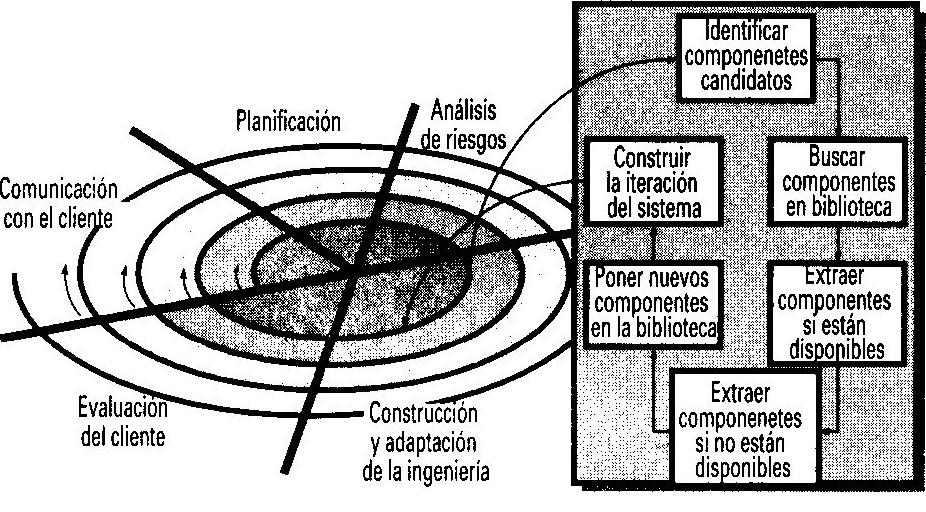
\includegraphics[width=17cm]{Imagenes/Modelo_componentes.jpeg}
	\caption{Diagrama mostrando el flujo iterativo y evolutivo de las etapas consideradas por la Metodología basada en el desarrollo por Componentes}
	\label{Metodologia_componentes}
\end{figure}

\newpage
\hfill \break
{\fontsize{12}{14}\textbf{6. Cronograma}}
\hfill \break
\justifying
\begin{longtable}{|p{2.5cm}|c|c|c|c|c|c|c|c|c|c|c|c|}
	\hline
	Actividades & Ago & Sep & Oct & Nov & Dic & Ene & Feb & Mar & Abr & May & Jun & Jul \\ \hline
	Investigación en dispositivo sensor y acelerómetro integrado & X &  & & & & & & & & & & \\ \hline
	Investigación en algoritmo DTW y optimización de este & X &  & & & & & & & & & & \\ \hline
	Investigación en modelos clasificadores de IA & X & X & & & & & & & & & & \\ \hline
	Análisis del prototipo \textit{wearable} &  & X & & & & & & & & & & \\ \hline
	Análisis del modelo clasificador &  & X & X & & & & & & & & & \\ \hline
	Diseño alto nivel del prototipo \textit{wearable} &  &  & X && & & & & & & & \\ \hline
	Diseño alto nivel del modelo clasificador &  &  & X &  & & & & & & & & \\ \hline
	Diseño del código motriz propuesto &  &  & X & X & & & & & & & & \\ \hline
	Diseño detallado del prototipo \textit{wearable} &  &  &  & X & & & & & & & & \\ \hline
	Diseño detallado del modelo clasificador \textit{wearable} &  &  &  & X & X & & & & & & & \\ \hline
	Especificación componentes lógicos del sistema &  &  &  &  & X & & & & & & & \\ \hline
	Evaluación TT I &  &  &  &  & X & X & & & & & & \\ \hline
	Ensamblado del prototipo de guante \textit{wearable} &  &  &  &  &  & X & X & & & & & \\ \hline
	Pruebas del funcionamiento del prototipo \textit{wearable} &  &  &  &  &  &  & X & & & & & \\ \hline
	Desarrollo de los componentes lógicos en el nodo sensor &  &  &  &  &  &  & X & X & & & & \\ \hline
	Implementación componentes y modelo para la clasificación de los patrones de movimiento &  &  &  &  &  &  & X & X & X & & & \\ \hline
	Desarrollo y configuración de componentes para la traducción \textit{Text-to-Speech} &  &  &  &  &  &  &  &  & X & X & & \\ \hline
	Pruebas unitarias en los componentes lógicos &  &  &  &  &  &  & X & X & X & X & & \\ \hline
	Pruebas de integración de los componentes &  &  &  &  &  &  &  & X & X & X & & \\ \hline
	Pruebas del sistema &  &  &  &  &  &  &  &  &  & X & X & \\ \hline
	Pruebas de aceptación por el usuario &  &  &  &  &  &  &  &  &  &  & X & X \\ \hline
	Generación de un artículo con la solución &  &  & X & X & X & X & X & X & X & X & X & \\ \hline
	Documentación del proyecto & X & X & X & X & X & X & X & X & X & X & X & X \\ \hline
	Evaluación TT II &  &  &  &  &  &  &  &  &  &  & X & X\\ \hline
\end{longtable}


\newpage
\hfill \break
{\fontsize{12}{14}\textbf{7. Referencias}}

\hfill \break
\begin{tabular}{p{0.5cm} p{17cm}}
	\text{[1]} & C. J .G. Ayala Aburto, "Guante traductor de señas para sordomudos," Tésis título licenciatura, ESIME, unidad Azcapotzalco,. Ciudad de México, México, 2018. \\ \\
	
	\text{[2]} & E. D. Jiménez Carbajal, G. E. Rivera Taboada, "Sistema de comunicación auditiva para personas con problemas del habla", Tésis para título de licenciatura, ESCOM, Ciudad de México, México, 2013. \\ \\
	
	\text{[3]} & D. Vishal, H. M. Aishwarya, K. Nishkala, B. T. Royan and T. K. Ramesh, "Sign Language to Speech Conversion,"(en inglés) 2017 IEEE International Conference on Computational Intelligence and Computing Research (ICCIC), 2017, pp. 1-4, doi: 10.1109/ICCIC.2017.8523832. \\ \\
	
	\text{[4]} & M. M. Chandra, S. Rajkumar and L. S. Kumar, "Sign Languages to Speech Conversion Prototype using the SVM Classifier," TENCON 2019 - 2019 IEEE Region 10 Conference (TENCON), 2019, pp. 1803-1807, doi: 10.1109/TENCON.2019.8929356. \\ \\
	
	\text{[5]} & N. Marques, "¿Qué es el lenguaje?," \textit{Babbel}, 02, 2018 [En línea]. Disponible en https://es.babbel.com/es/magazine/que-es-lenguaje \\ \\
	
	\text{[6]} & "Presentación de Resultados," INEGI Censo 2020., México, 2020. [En línea]. Disponible en https://www.inegi.org.mx/contenidos/programas/ccpv/2020/doc/Censo2020\_Principales\_resultados\_EUM.pdf \\ \\
	
	\text{[7]} & O. Castillero Mimenza, "Los 8 tipos de trastornos del habla," \textit{Psicología y Mente}. [En línea]. Disponible en https://psicologiaymente.com/clinica/tipos-trastornos-habla \\ \\
	
	\text{[8]} & National Institute on Deafness and Other Communication Disorders,(2017, 03. 06). "La afasia".[En línea]. Disponible en https://www.nidcd.nih.gov/es/espanol/afasia \\ \\
	
	\text{[9]} & A. Triglia, "Afasias:los principales trastornos del lenguaje," \textit{Psicología y Mente}. [En línea]. Disponible en https://psicologiaymente.com/clinica/afasias-trastornos-lenguaje  \\ \\
	
	\text{[10]} & "Afasia de Broca," National Aphasia Association.[En línea]. Disponible en https://www.aphasia.org/es/afasia-de-broca/ \\ \\
	
	\text{[11]} & "Apraxia", \textit{Instituto Nacional de Trastornos Neurológicos y Accidentes Cerebrovasculares}. 03, 2022.[En línea]. Disponible en https://espanol.ninds.nih.gov/es/trastornos/apraxia \\ \\
	
	\text{[12]} & J. Huang, "Apraxia," \textit{MSD}. 10, 2021.[En línea]. Disponible en https://www.msdmanuals.com/es-mx/hogar/enfermedades-cerebrales,-medulares-y-nerviosas/disfunci\%C3\%B3n-cerebral/apraxia \\ \\
	
	\text{[13]} & "La Disartria," \textit{American Speech Language Hearing Association}.[En línea]. Disponible en https://www.asha.org/public/speech/Spanish/La-Disartria/ \\ \\
	
	\text{[14]} & J. Huang, "Disartria," \textit{MSD}. 10, 2021.[En línea]. Disponible en https://www.msdmanuals.com/es-mx/hogar/enfermedades-cerebrales,-medulares-y-nerviosas/disfunci\%C3\%B3n-cerebral/disartria \\ \\
	
	\text{[15]} &  INEGI (2020).[En línea]. Disponible en https://www.inegi.org.mx/temas/educacion/ \\ \\
	
\end{tabular}

\newpage

{\fontsize{12}{14}\textbf{8. Alumnos y Directores}}

\begin{multicols*}{2}
	\hfill \break
	\hfill \break
	\justifying
	\textit{Luis Eduardo Valle Martínez}.- Alumno de la carrera de Ing. en Sistemas Computacionales en ESCOM, Especialidad Sistemas, Boleta: 2015090780, Tel. 5566143276, email: lvallem1400@alumno.ipn.mx
	
	\hfill \break
	\hfill \break
	\centering
	
\includegraphics[width=5cm]{Imagenes/firma.png}
	
	
	Firma: \hrulefill
	
	\hfill \break
	\hfill \break
	\justifying
	\textit{Rodolfo Romero Herrera}.- Profesor de tiempo completo Laboratorio de posgrado Sistemas computacionales móviles. Candidato a Doctor en ciencias en Comunicaciones y Electrónica. Maestría en ciencias en Ingeniería electrónica. Ingeniería en comunicaciones y Electrónica. Área de trabajo Inteligencia Artificial y Procesamiento digital de señales. Tel. 5535216128, email: rromeroh@ipn.mx.
	
	\hfill \break
	\centering
	
\includegraphics[width=5cm]{Imagenes/firma_Rodolfo_Romero.png}
	
	Firma: \hrulefill
	
	\hfill \break
	\hfill \break
	\justifying
	\textit{Jesús Yaljá Montiel Pérez}.- Profesor de tiempo completo adscrito al Laboratorio de Robótica y Mecatrónica del Centro de Investigación en Computación del Instituto Politécnico nacional. Doctor en comunicaciones y electrónica. Maestro en Ciencias en Ingeniería electrónica e Ingeniero Físico. Sus intereses son: la Inteligencia Artificial, sensores y robótica. Tel: 5524940919, Ext. IPN: 56665, email: yalja@ipn.mx
	
	\hfill \break
	\hfill \break
	\centering
	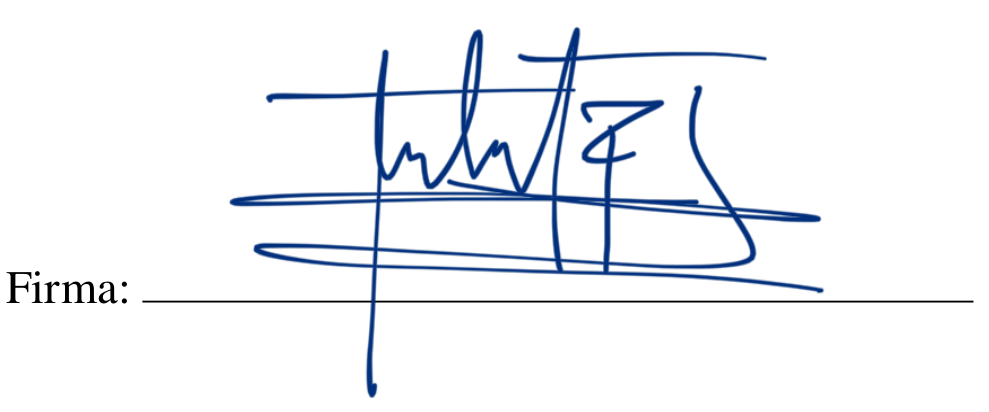
\includegraphics[width=7.9cm]{Imagenes/firma_Jesus_Yalja.png}

	
	
	\begin{tabular}{>{\raggedleft\arraybackslash\columncolor[HTML]{EFEFEF}}p{6.8cm}}
		{\scriptsize CARÁCTER: Confidencial}\\
		{\scriptsize FUNDAMENTO LEGAL: Artículo 11 Fracc. V y Artículos 108, 113 y 117 de la Ley Federal de Transparencia y Acceso} \\
		{\scriptsize a la Información Pública.}\\
		{\scriptsize PARTES CONFIDENCIALES: Número de boleta y teléfono}
	\end{tabular}

\end{multicols*}

\end{document}
